\section{Auswertung}
\label{sec:auswertung}

In dem Versuch wird die Molwärme $C\ua{p}$ nach Formel \eqref{eq:c_p}
bestimmt. Tabelle \ref{tab:c_p} zeigt die Ergebnisse der
Wärmekapazität $C\ua{p}$ für verschiedene Temperaturen.


\import{Tabellen/C_p.tex}

\section{Wärmekapazität $C\ua{V}$}

Aus der Wärmekapazität bei konstantem Druck $C\ua{p}$ kann
durch den Zusammenhang \eqref{eqn:c_p-c_v} berechnet werden.
Der Verlauf der aus den Messdaten errechneten Wärmekapazität $C\ua{V}$
für verschiedene Temperaturen $T$ ist in Abb. \ref{fig:c_v} dargestellt.

\begin{figure}
  \centering
  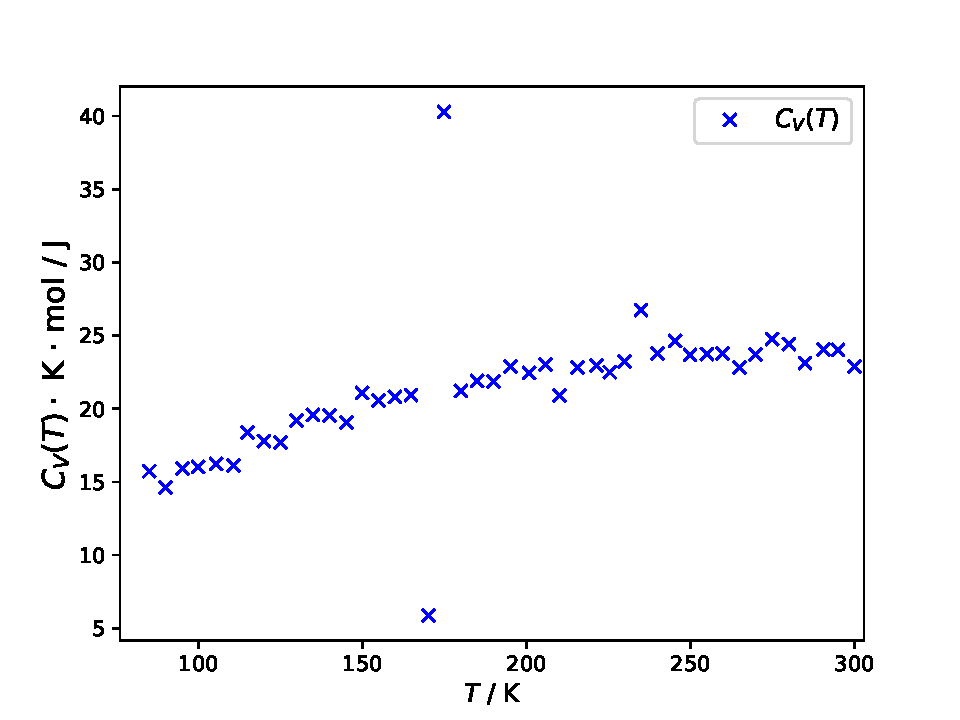
\includegraphics{Plots/C_V.pdf}
  \caption{Daten der Wärmekapazität für steigende Temperaturen.}
  \label{fig:c_v}
\end{figure}

Es wird ersichtlich, dass in Abb. \ref{fig:c_v} Werte auftauchen, die sehr
stark erwarteten Trend abweichen.
Diese Abweichung wird auf zwei vermutlich fehlerhafte Messdaten zurückgeführt.
Eine Darstellung von $C\ua{V}$ ohne diese beiden Messdaten ist in Abb. \ref{fig:c_v_korrektur}
einzusehen.

\begin{figure}
  \centering
  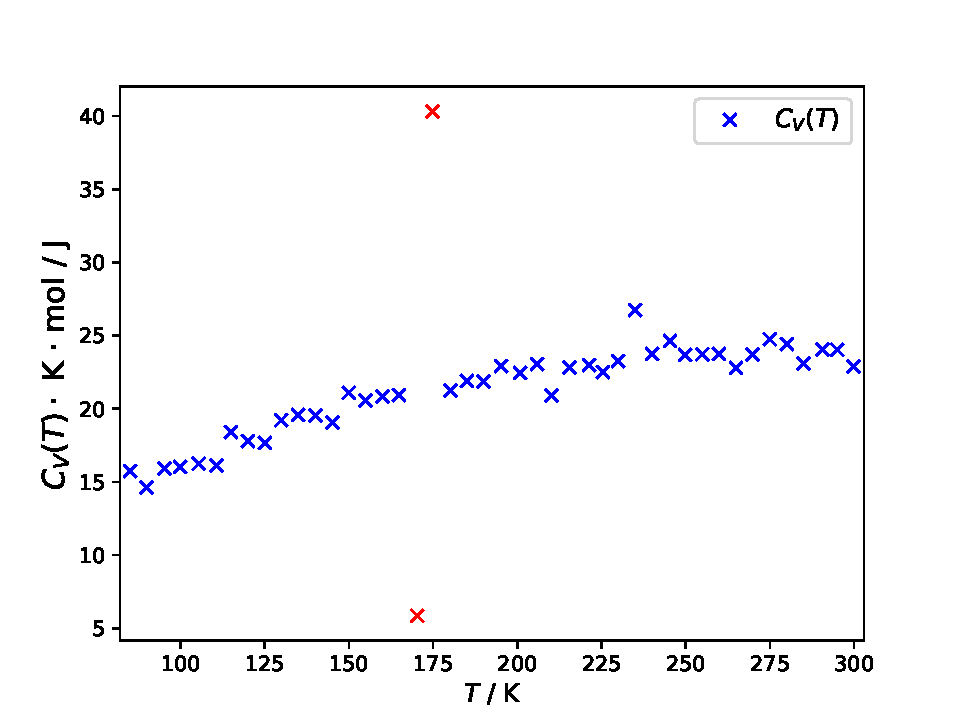
\includegraphics{Plots/C_V_korrektur.pdf}
  \caption{Angepasste Daten der Wärmekapazität für steigende Temperaturen.}
  \label{fig:c_v_korrektur}
\end{figure}

\section{Diskussion}
\label{sec:diskussion}
